
\documentclass[xcolor={dvipsnames}]{beamer}
\usepackage{amsmath,amsfonts,amssymb,pxfonts,eulervm,xspace}
\usepackage{graphicx}
 \usepackage{multimedia}
\usepackage{media9}
\usepackage{tabularx}
\usepackage{minted}

\graphicspath{{./figures/}}
\usetheme{ccnycrest}


\newenvironment{changemargin}[2]{%
\begin{list}{}{%
\setlength{\topsep}{0pt}%
\setlength{\leftmargin}{#1}%
\setlength{\rightmargin}{#2}%
\setlength{\listparindent}{\parindent}%
\setlength{\itemindent}{\parindent}%
\setlength{\parsep}{\parskip}%
}%
\item[]}{\end{list}}

\begin{document}

\title{ CS102: Constants, Math, Formatting}
\author{Hannah Aizenman}

\begin{frame}
	\titlepage
\end{frame}

\begin{frame}[fragile]{Symbolic Constants}
\center
\begin{minted}{c++}
	const double PI = 3.1416;
	const double DEG_TO_RAD = PI/180.0;
	const float AVOGADRO = 6.022e23;
	const int MAXIMUM = 100;
	const string CLASS = "CS102";
\end{minted}

\begin{block}{}
	\begin{itemize}
		\item \textbf{const} means value of var is never changed
		\item used for math/science constants
		\item also used for \textbf{magic numbers}
		\item ALL CAPS by convention
	\end{itemize}
\end{block}
\end{frame}

\begin{frame}[fragile]{Math Library}
	\center
	\huge How do we compute \\the area of a circle? 
	\pause
	\begin{equation*}
	area = \pi r^2
	\end{equation*}
	\pause
	\begin{minted}{c++}
	const double PI = 3.1416;
	double area = PI*??;
	\end{minted}
\end{frame}



\begin{frame}{Math Library}
\begin{figure}
	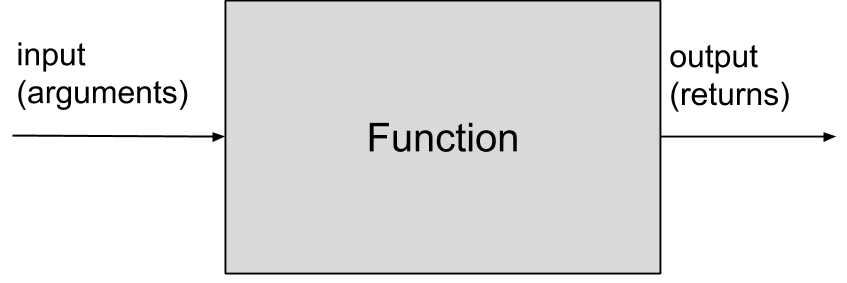
\includegraphics[width=1\textwidth]{function}
\end{figure}
\pause
\begin{block}{Math Equivalent}
\begin{equation*}
	f(x) = y
\end{equation*}
\center
\textbf{x} is the \textbf{input}\\
\textbf{y} is the \textbf{output}
\end{block}
\end{frame}


\begin{frame}[fragile]{Using the Math Library}
\begin{minted}{c++}
#include <iostream>
#include <cmath> //math library

using namespace std;

int main(){
    const double PI = 3.1416;
    int r = 10;
    //pow is in the math library;
    double area = PI*pow(r,2.0);
    cout<<"Area: "<<area<<endl;
    return 0;
}
\end{minted}
\end{frame} 

\begin{frame}[fragile]{Better Output}
\begin{minted}{c++}
#include <iomanip>//library for formatting output
    //...code
    cout<<"Area: "<<setprecision(3)<<area<<endl;
   //...more code
\end{minted}

\begin{block}{}
	\begin{itemize}
		\item formatters need to come before what they're formatting
		\item setprecision specifies 3 decimal points
	\end{itemize}
\end{block}
\end{frame}

\begin{frame}{Format Flags}
http://glasslab.engr.ccny.cuny.edu/u/hannah/cs102/cs102L3.pdf
\end{frame}
\end{document}